\documentclass[UTF8]{ctexart}

\usepackage{ctex}
\CTEXsetup[format={\Large\bfseries}]{section}
\usepackage[top=28mm,bottom=28mm,left=15mm,right=15mm]{geometry}

\usepackage{fancyhdr}
\fancypagestyle{plain}{\pagestyle{fancy}}
\pagestyle{fancy}
\lhead{\kaishu 清华大学药学院药理毒理实验}
\newcommand{\numOfReport}[1]{\rhead{\kaishu 实验报告#1}}

\usepackage{fontspec}
\usepackage{wasysym}
\setCJKmainfont[AutoFakeBold={2}]{STZhongsong}
\setCJKmonofont{STZhongsong}

\usepackage{float}
\usepackage{booktabs}
\usepackage{tabularx}
\usepackage{array}
\usepackage{amsmath}
\usepackage{amsfonts}
\usepackage{amssymb}
\usepackage[figuresleft]{rotating}
\usepackage[para]{threeparttable}
\newcommand\info[2][40mm]{\underline{\makebox[#1][c]{#2}}}
\newcommand{\infoTable}[7]{
    \renewcommand\arraystretch{1.4}
    \begin{table}
        \begin{tabularx}{\textwidth}{
        >{\hsize=0.6\hsize\linewidth=\hsize}X
        >{\hsize=0.6\hsize\linewidth=\hsize}X
        >{\hsize=2.0\hsize\linewidth=\hsize}X
        >{\hsize=0.8\hsize\linewidth=\hsize}X
        }
            天气:\info[14mm]{#1} & 温度:\info[14mm]{#2 $^{\circ}\text{C}$} & 湿度:\info[14mm]{#3 $\%$} & 日期:#4\\
            姓名:\info[14mm]{#5} & 班级:\info[14mm]{#6} & 同组人:\info[70mm]{#7} & 
        \end{tabularx}
    \end{table}
}
\newcommand\columnC{\centering\arraybackslash}
\newcommand\columnL{\raggedright\arraybackslash}
\newcommand\columnR{\raggedleft\arraybackslash}

\usepackage{svg}
\usepackage{pdfpages}
\title{盐酸普鲁卡因 $\text{LD}_{50}$ 的测定}
\author{}
\numOfReport{二}

\begin{document}
\infoTable{晴}{23}{80}{9/18/2024}{何昱晖}{药3}{荣子健、马逸然、赵方一澜}
\date{}
\maketitle

\section{实验目的和原理}

\subsection{实验目的}

\begin{itemize}
    \item [(1)] 掌握测定药物盐酸普鲁卡因 $\text{LD}_{50}$ 的方法、实验步骤和计算过程;
    \item [(2)] 了解药物急性毒性实验的意义,以及药物安全性评价的主要指标。
\end{itemize}

\subsection{实验原理}

\subsubsection{$\text{LD}_{50}$}

质反应量效曲线的横坐标为对数剂量,而纵坐标采用阳性反应发生的频数时,一般为正态分布曲线。如改用累加阳性频数为纵坐标时,可以得到标准的 S 型曲线。该曲线的中央部分($50\%$ 反应处)接近一条直线,斜率最大,其相应的剂量也就是能使群体中半数个体出现某一效应的剂量,通常称为半数效应量。如效应为疗效,则称半数有效量($\text{ED}_{50}$);如效应为死亡,则称半数致死量($\text{LD}_{50}$)。这些数值是评价药物作用强度和药物安全性的重要参数。\textbf{$\text{ED}_{50}$ 数值越小,药物的作用越强;$\text{LD}_{50}$ 越小,则药物的毒性越大}。

$\text{LD}_{50}$ 的测定方法很多,寇式法、图解法、概率法等。本实验采用改良寇式法。此法设计简单、计算方便、要求不高,但精度不够,一般用于毒性的初步测定。改良寇式法取小鼠随机分组、编号、称重。各组按等比剂量分别腹腔注射盐酸普鲁卡因溶液,记录各组动物死亡数,列表统计 $p$ 值。按公式

$$
    \text{LD}_{50}=\lg^{-1}\left[\chi_m-\mathrm{i}\left(\sum_{k=1}^np_k-0.5\right)\right]
$$

其中

\begin{itemize}
    \item [$\chi_m$:]最大剂量组剂量对数;
    \item [$\mathrm{i}$:]相邻两组剂量高剂量与低剂量比的对数(相邻两组对数剂量的差值);
    \item [$p_k$:]各组动物的死亡率,用小数表示;
    \item [$n$:]每组动物数。
\end{itemize}

设 $\text{LD}_{50}$ 的 $95\%$ 可信限为 $t$,则

$$
    t=\lg^{-1}\left[\lg\text{LD}_{50}\pm 1.96\mathrm{i}\sqrt{\frac{\sum_{k=1}^{n}(p_k-p_k^2)}{n-1}}\right]
$$

\subsubsection{盐酸普鲁卡因}

盐酸普鲁卡因(化学式 $\text{C}_{13}\text{H}_{21}\text{Cl}\text{N}_2\text{O}_2$),是一种局麻药,作用于外周神经产生传导阻滞作用,依靠浓度梯度以弥散方式穿透神经细胞膜,在内侧阻断钠离子通道,使神经细胞兴奋阈值升高,丧失兴奋性和传导性,信息传递被阻断,具有良好的局部麻醉作用。

\section{实验材料}

\begin{itemize}
    \item 实验器材:天平、注射器(1 mL)、鼠盒;
    \item 实验动物:ICR 小鼠,体重 $18\sim 22\text{g}$,雌雄兼用;
    \item 实验药品:系列浓度盐酸普鲁卡因溶液;
    \item 其它试剂:生理盐水。
\end{itemize}

\section{实验方法}

每组各 12 只小鼠,雌雄各半,称重,标记。腹腔注射药物。根据实验结果计算相邻剂量的比值为 $1:0.8$,给药剂量分别为 $102.4$、$128$、$160$、$200$、$250$、$312\text{mg}/\text{kg}$。按 $0.1\text{mg}/\text{g}$ 体重给予小鼠腹腔注射不同浓度的盐酸普鲁卡因溶液。给药后,观察小鼠的行为学情况,记录小鼠出现死亡时的症状和时间。一般未死亡的小鼠经 $15\sim 30\text{min}$ 将恢复正常。故只需观察 $30\text{min}$ 内小鼠的死亡数。

\newpage

\section{实验结果}

以下表 1 和表 2 是我组的观察结果:

\begin{table}[H]
    \centering
    \begin{threeparttable}[b]
        \caption{盐酸普鲁卡因 $\text{LD}_{50}$ 的测定——本组数据}
        \quad

        \begin{tabularx}{\textwidth}{
            >{\columnC\hsize=0.5\hsize\linewidth=\hsize}X
            >{\columnC\hsize=0.5\hsize\linewidth=\hsize}X
            >{\columnC\hsize=0.5\hsize\linewidth=\hsize}X
            >{\columnC\hsize=0.5\hsize\linewidth=\hsize}X
            >{\columnC\hsize=0.5\hsize\linewidth=\hsize}X
            >{\columnC\hsize=3\hsize\linewidth=\hsize}X
            >{\columnC\hsize=0.5\hsize\linewidth=\hsize}X
        }
            \toprule[1.5pt]
            组别 & 给药剂量\tnote{1} & 小鼠性别 & 小鼠体重\tnote{2} & 给药量\tnote{3} & 给药后小鼠行为学情况 &  是否死亡\\
            \midrule
            1 & 102.4 & \female & 23 & 0.23 & 给药后正常爬动;1-3min 内有较多次理毛和舔舐腹部行为;于 5min 左右稍显安静,但爬动与探索鼠盒行为正常;30min 内呼吸正常且仍能以前肢攀爬鼠盒并用后肢支撑起身体;最终未死亡 & $-$\\
            \midrule
            2 & 102.4 & \male & 25 & 0.25 & 给药后正常爬动;1-3min 内较为安静,6min 开始有自由行动;最终未死亡 & $-$ \\
            \midrule
            3 & 128 & \female & 26 & 0.26 & 给药后正常爬动;约 4min 时出现后肢无力、拖行爬行现象;6min 后无法正常爬动,改为身体较为瘫软的趴卧状态,呼吸频率较快;安静趴卧时间持续约 10min,后恢复缓慢爬动,约 20min 时可以短暂用前肢攀爬鼠盒并用后肢支撑起身体;最终未死亡 & $-$ \\
            \midrule
            4 & 128 & \male & 23 & 0.23 & 给药后正常爬动,爬动频率低,5min 开始尾巴呈翘起状态,变为安静少动;最终未死亡 & $-$ \\
            \midrule
            5 & 160 & \female & 24 & 0.24 & 给药后安静少动,步态蹒跚,且后肢无力、向身体两侧摊开的表现;5-10min 眯眼闭目,尾巴变白;最终死亡 & $+$ \\
            \midrule
            6 & 160 & \male & 25 & 0.25 & 给药后缓慢爬动;约 2min 时出现后肢无力、向身体两侧摊开的表现;3min 大幅抽搐,举前肢抓挠空气并竖直尾巴,同时有“青蛙跳”行为;5-10min 完全不能正常支撑身体,与鼠盒内8号小鼠相互依靠支撑身体,呼吸频率较快且比较艰难;约 18min 开始近正常爬动;22-27min 静趴,后恢复完全正常,最终未死亡 & $-$ \\
            \bottomrule[1.5pt]
        \end{tabularx}
        \begin{tablenotes}
            \item [1] 单位 $\text{mg}/\text{kg}$
            \item [2] 单位 $\text{g}$
            \item [3] 单位 $\text{mL}$
        \end{tablenotes}
    \end{threeparttable}
\end{table}

\begin{table}[H]
    \centering
    \begin{threeparttable}[b]
        \caption{盐酸普鲁卡因 $\text{LD}_{50}$ 的测定——本组数据(续表)}
        \quad

        \begin{tabularx}{\textwidth}{
            >{\columnC\hsize=0.5\hsize\linewidth=\hsize}X
            >{\columnC\hsize=0.5\hsize\linewidth=\hsize}X
            >{\columnC\hsize=0.5\hsize\linewidth=\hsize}X
            >{\columnC\hsize=0.5\hsize\linewidth=\hsize}X
            >{\columnC\hsize=0.5\hsize\linewidth=\hsize}X
            >{\columnC\hsize=3\hsize\linewidth=\hsize}X
            >{\columnC\hsize=0.5\hsize\linewidth=\hsize}X
        }
            \toprule[1.5pt]
            组别 & 给药剂量\tnote{1} & 小鼠性别 & 小鼠体重\tnote{2} & 给药量\tnote{3} & 给药后小鼠行为学情况 &  是否死亡\\
            \midrule
            7 & 200 & \female & 24 & 0.24 & 给药后正常爬动;1min 半变为静趴;2min 半竖直尾巴开始抽搐,反应剧烈有跳跃行为;3min 开始举前肢抓挠摆动并持续抽搐;5min 转为侧躺,继续剧烈抽搐直到7min;8min 时仅余小幅度心跳;至 9min 无反应,触摸无心跳,确认死亡 & $+$ \\
            \midrule
            8 & 200 & \male & 23 & 0.23 & 给药后正常爬动,有理毛行为;2min 半后开始小幅抽动,可观察到后腿无力呈现拖行行态;3min 大幅抽搐,举前肢抓挠空气并竖直尾巴;4min 半稍缓为原地抖动;5min 可观察到心跳剧烈,行动力减弱但持续左顾右盼;6min 开始再度挺尾,抽搐并挣动,间断性发生直到 11min 逐渐平缓;15min 开始近正常爬动;20min 静趴,后恢复完全正常 & $-$ \\
            \midrule
            9 & 250 & \female & 23 & 0.23 & 给药后缓慢爬动,有理毛行为;1min 至 1min 半时竖起尾巴持续抽搐;2min 半趴下完全不动,翻过后无反应,触摸无心跳,确认死亡 & $+$ \\
            \midrule
            10 & 250 & \male & 24 & 0.24 & 给药后缓慢爬动,1min 后变为静趴;1min 半至 2min 间竖起尾巴持续抽搐;3min 复又趴下,心跳微弱;5min 时静止不动,翻过后无反应,触摸无心跳,确认死亡 & $+$ \\
            \midrule
            11 & 312 & \female & 24 & 0.24 & 给药 2min 后竖起尾巴并抖动一周;3min 后侧趴并持续抽搐,可见明显心跳;3min 半时心跳减弱;4min 半有静止不动,触摸无反应无心跳,确认死亡 & $+$ \\
            \midrule
            12 & 312 & \male & 25 & 0.25 & 给药 1min 时静趴,可观察到心跳;2min 后蹒跚爬动;3min 后进入半侧躺状态,呼吸变微弱;5min 半时完全不动,翻过后无反应,触摸无心跳,确认死亡 & $+$ \\
            \bottomrule[1.5pt]
        \end{tabularx}
        \begin{tablenotes}
            \item [1] 单位 $\text{mg}/\text{kg}$
            \item [2] 单位 $\text{g}$
            \item [3] 单位 $\text{mL}$
        \end{tablenotes}
    \end{threeparttable}
\end{table}

\begin{table}[H]
    \centering
    \caption{盐酸普鲁卡因 $\text{LD}_{50}$ 的测定——全班数据}
    \quad

    \begin{tabularx}{\textwidth}{
        >{\columnC\hsize=1\hsize\linewidth=\hsize}X
        >{\columnC\hsize=1\hsize\linewidth=\hsize}X
        >{\columnC\hsize=1\hsize\linewidth=\hsize}X
        >{\columnC\hsize=1\hsize\linewidth=\hsize}X
        >{\columnC\hsize=1\hsize\linewidth=\hsize}X
    }
        \toprule[1.5pt]
        组别 & 剂量(mg/kg) & 每组只数 & 死亡动物数 & 死亡率\\
        \midrule
        1 & 102.4 & 12 & 0 & $0\%$ \\
        \midrule
        2 & 128 & 12 & 0 & $0\%$ \\
        \midrule
        3 & 160 & 12 & 3 & $25\%$ \\
        \midrule
        4 & 200 & 12 & 6 & $50\%$ \\
        \midrule
        5 & 250 & 12 & 11 & $91.67\%$ \\
        \midrule
        6 & 312 & 12 & 12 & $100\%$ \\
        \bottomrule[1.5pt]
    \end{tabularx}
\end{table}

$$
    \text{LD}_{50}=\lg^{-1}\left(\lg 312-\lg 1.25\times\left(\frac{32}{72}-0.5\right)\right)=315.89\text{mg}\cdot\text{kg}^{-1}
$$

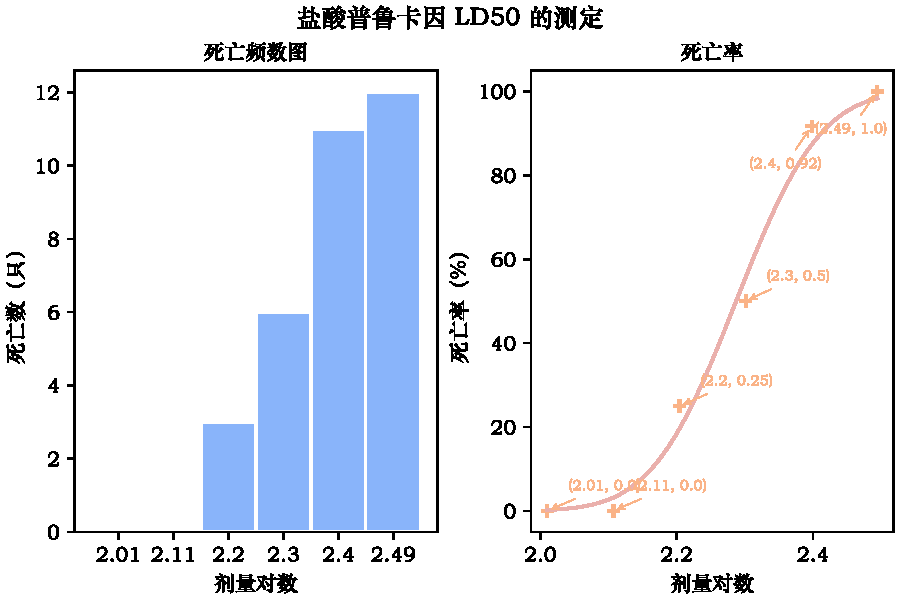
\includepdf[page=1]{figure-2_svg.pdf}
\end{document}